\section{Wyznaczenie odpowiedzi skokowej procesu}

Początkowy sygnał sterujący G1 ustalono w punkcie pracy $U=32$. 
Przeprowadzone zostały trzy skoki sterowania: na wartości $U_{1}=35$, $U_{2}=44$, $U_{3}=55$. 
Uzyskane odpowiedzi skokowe dla tych zmian sygnału zostały przedstawione na poniższym rysunku.

\begin{figure}[H]
    \centering
    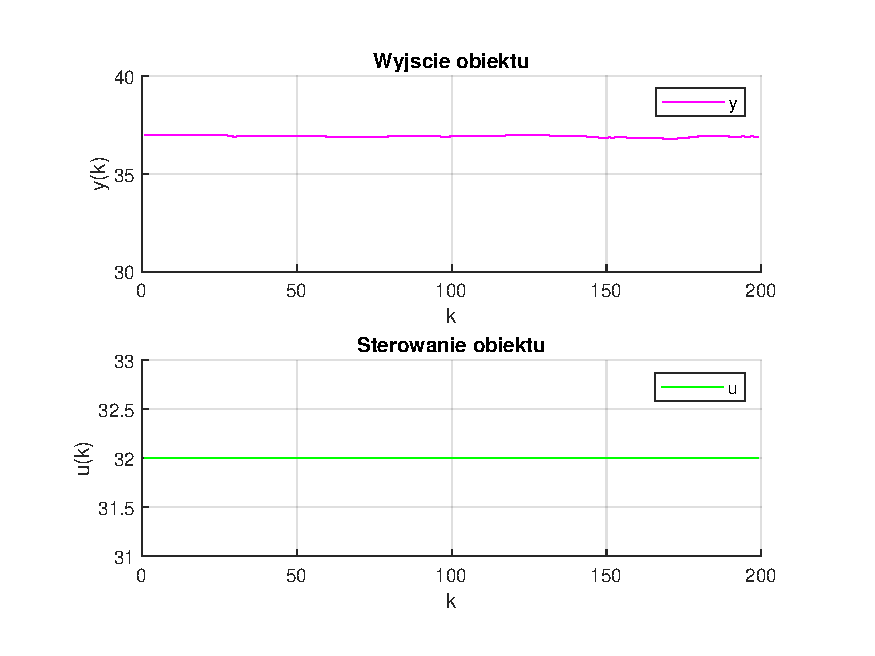
\includegraphics[scale=0.90]{../lab/zad_1/y.pdf}
    \caption{Punkt pracy obiektu}
\end{figure}


Właściwości statyczne obiektu zostały określone z wykresu charakterystyki statycznej, 
który utworzony został na podstawie serii odpowiedzi skokowych. 

\begin{figure}[H]
    \centering
    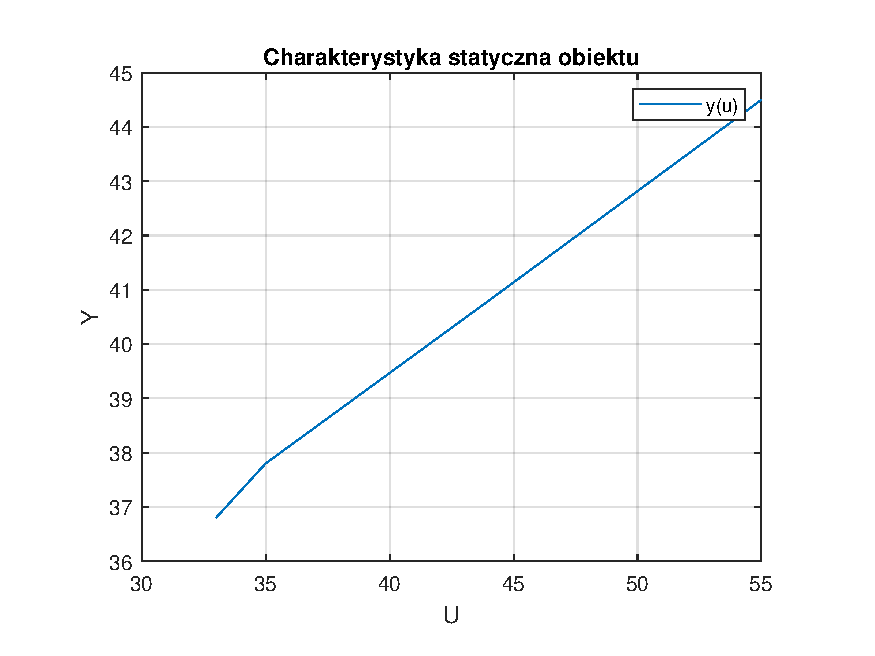
\includegraphics[scale=0.90]{../lab/zad_2/char_stat.pdf}
    \caption{Punkt pracy obiektu}
\end{figure}

Właściwości statyczne obiektu są w przybliżeniu liniowe, 
można więc wyznaczyć wzmocnienie statyczne procesu, 
które równe jest nachyleniu wykresu charakterystyki statycznej $K=\num{0.8073}$.
